%% beamer/knitr slides
%% for Statistical Modeling and Data Visualization course @ UMass
%% Nicholas Reich: nick [at] schoolph.umass.edu


\documentclass[table]{beamer}\usepackage[]{graphicx}\usepackage[]{color}
% maxwidth is the original width if it is less than linewidth
% otherwise use linewidth (to make sure the graphics do not exceed the margin)
\makeatletter
\def\maxwidth{ %
  \ifdim\Gin@nat@width>\linewidth
    \linewidth
  \else
    \Gin@nat@width
  \fi
}
\makeatother

\definecolor{fgcolor}{rgb}{0.345, 0.345, 0.345}
\newcommand{\hlnum}[1]{\textcolor[rgb]{0.686,0.059,0.569}{#1}}%
\newcommand{\hlstr}[1]{\textcolor[rgb]{0.192,0.494,0.8}{#1}}%
\newcommand{\hlcom}[1]{\textcolor[rgb]{0.678,0.584,0.686}{\textit{#1}}}%
\newcommand{\hlopt}[1]{\textcolor[rgb]{0,0,0}{#1}}%
\newcommand{\hlstd}[1]{\textcolor[rgb]{0.345,0.345,0.345}{#1}}%
\newcommand{\hlkwa}[1]{\textcolor[rgb]{0.161,0.373,0.58}{\textbf{#1}}}%
\newcommand{\hlkwb}[1]{\textcolor[rgb]{0.69,0.353,0.396}{#1}}%
\newcommand{\hlkwc}[1]{\textcolor[rgb]{0.333,0.667,0.333}{#1}}%
\newcommand{\hlkwd}[1]{\textcolor[rgb]{0.737,0.353,0.396}{\textbf{#1}}}%
\let\hlipl\hlkwb

\usepackage{framed}
\makeatletter
\newenvironment{kframe}{%
 \def\at@end@of@kframe{}%
 \ifinner\ifhmode%
  \def\at@end@of@kframe{\end{minipage}}%
  \begin{minipage}{\columnwidth}%
 \fi\fi%
 \def\FrameCommand##1{\hskip\@totalleftmargin \hskip-\fboxsep
 \colorbox{shadecolor}{##1}\hskip-\fboxsep
     % There is no \\@totalrightmargin, so:
     \hskip-\linewidth \hskip-\@totalleftmargin \hskip\columnwidth}%
 \MakeFramed {\advance\hsize-\width
   \@totalleftmargin\z@ \linewidth\hsize
   \@setminipage}}%
 {\par\unskip\endMakeFramed%
 \at@end@of@kframe}
\makeatother

\definecolor{shadecolor}{rgb}{.97, .97, .97}
\definecolor{messagecolor}{rgb}{0, 0, 0}
\definecolor{warningcolor}{rgb}{1, 0, 1}
\definecolor{errorcolor}{rgb}{1, 0, 0}
\newenvironment{knitrout}{}{} % an empty environment to be redefined in TeX

\usepackage{alltt}


%       ************************************************
%       **        LaTeX preamble to be used with all 
%	**        statsTeachR labs/handouts.
%
%	Author: Nicholas G Reich
%	Last modified: 14 January 2014
%	************************************************

% \documentclass[table]{beamer}

%	Set theme (a nice plain one)
\usetheme{Malmoe}

%	Use named colors, set main color of theme
%		to match Web site color:
\definecolor{MainColor}{RGB}{10, 74, 109}
\colorlet{MainColorMedium}{MainColor!50}
\colorlet{MainColorLight}{MainColor!20}
\usecolortheme[named=MainColor]{structure} 

%	For tables
%[dvipsnames] [table]
\usepackage{xcolor}

%% calling tabu.sty, assuming a particular directory structure
\usepackage{../../slide-includes/tabu}	% Even fancier than tabulary
\usepackage{multirow}

%	Just for the degree symbol
\usepackage{textcomp}

%	Get rid of footline (page, author, etc. on each slide)
\setbeamertemplate{footline}{}
%	Get rid of navigation buttons
\setbeamertemplate{navigation symbols}{}

%	Make footnotes not ugly
\usepackage{hanging}
\setbeamertemplate{footnote}{\raggedright\hangpara{1em}{1}\makebox[1em][l]{\insertfootnotemark}\footnotesize\insertfootnotetext\par}

%	Text style for code snippets inline in text:
\newcommand{\codeInline}[1]{\texttt{#1}}

%	Text style for emphasis stronger than \emph:
%		(Note, this doesn't toggle the way \emph does.
%			(Note, this can be done, didn't seem worth the trouble.))
\newcommand{\strong}[1]{{\bfseries{#1}}}


%        ******	Define title page	**********************
\setbeamertemplate{title page}{
	{\color{MainColor}
	% There must be a better way than this -vspace at
	%	 the top and bottom of the page to reduce the 
	%	 bottom margin, but I can't find one that works.
	\vspace{-6em}

% 	% Go to a lot of trouble to get the title in a
% 	%	nice box, since customizing a beamer block
% 	%	does not entirely work here (I don't know why)
	\newlength{\titleBoxWidth}
	\setlength{\titleBoxWidth}{\textwidth}
	\addtolength{\titleBoxWidth}{-2.0em}
	\setlength{\fboxsep}{1.0em}
	\setlength{\fboxrule}{0pt}
	\fcolorbox{MainColor!25}{MainColor!25}{
		\parbox{\titleBoxWidth}{
			\raggedright
			\LARGE\textbf{\inserttitle}
		}	% end parbox
	}	% end fcolorbox

	\vfill
	\small{Author: \insertauthor}
	\vspace{\baselineskip}

	\small{\Course}

	\small{\Instructor}
	\vspace{\baselineskip}

	%\small{\emph{This material is part of the \strong{statsTeachR} project}}

	\vspace{0.33\baselineskip}\scriptsize{\emph{\LicenseText}}


		\vspace{-15em}

	}	% end color
	\clearpage
}	% end define title page

%	The following variables are assumed by the standard preamble:
%	Global variable containing module name:
\title{Regression: dummy variables}
%	Global variable containing module shortname:
%		(Currently unused, may be used in future.)
\newcommand{\ModuleShortname}{introRegression}
%	Global variable containing author name:
\author{Nicholas G Reich}
%	Global variable containing text of license terms:
\newcommand{\LicenseText}{Made available under the Creative Commons Attribution-ShareAlike 3.0 Unported License: http://creativecommons.org/licenses/by-sa/3.0/deed.en\textunderscore US }
%	Instructor: optional, can leave blank.
%		Recommended format: {Instructor: Jane Doe}
\newcommand{\Instructor}{}
%	Course: optional, can leave blank.
%		Recommended format: {Course: Biostatistics 101}
\newcommand{\Course}{}


% leftovers from openintro slides



\input{../../slide-includes/shortcuts}
\usepackage{bbm}


%	******	Document body begins here	**********************
\IfFileExists{upquote.sty}{\usepackage{upquote}}{}
\begin{document}

%	Title page
\begin{frame}[plain]
	\titlepage
\end{frame}

%	******	Everything through the above line must be placed at
%		the top of any TeX file using the statsTeachR standard
%		beamer preamble.





%%%%%%%%%%%%%%%%%%%%%%%%%%%%%%%%%%%%%%%%%%

\begin{frame}{Outline}



\bi
  \myitem Dummy variables for categorical covariates
\ei

\end{frame}


%%%%%%%%%%%%%%%%%%%%%%%%%%%%%%%%%%%%%%%%%%
 %%%%%%%%%%%%%%%%%%%%%%%%%%%%%%%%%%%%%%%%%%



 %%%%%%%%%%%%%%%%%%%%%%%%%%%%%%%%%%%%%%%%%%

\begin{frame}{Categorical predictors}

\bi
	\myitem Assume $X$ is a categorical / nominal / factor variable with $k$ levels: e.g. `Industry'.
	\myitem If you use a single predictor with continuous values of $1, 2, \ldots, K$ this assumes that a ``one unit increase'' has a clear meaning.
	\myitem You need to create {\it indicator} or {\it dummy} variables so that each level stands on its own and can be estimated separately.
\ei

\centering
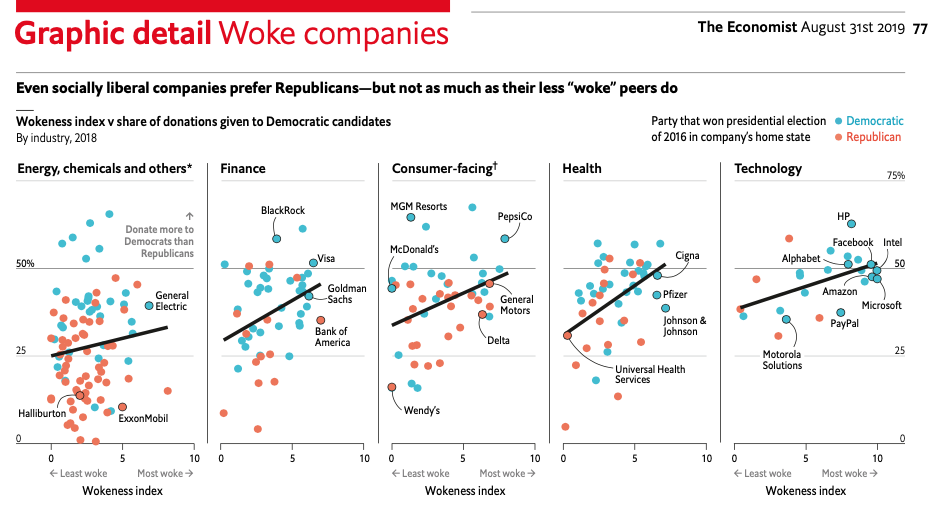
\includegraphics[width=.7\textwidth]{figure-static/woke-factors.png}

\end{frame}

 %%%%%%%%%%%%%%%%%%%%%%%%%%%%%%%%%%%%%%%%%%

\begin{frame}{Categorical predictors}

\begin{block}{Important to distinguish between...}
\bi
	\myitem  ``nominal'' categorical variables: e.g. ones with no natural ordering, such as Industry, country, etc...
	\myitem ``ordinal'' categorical variables: e.g. ones with a natural ordering, such as education level, or age grouping.
\ei
\end{block}

\end{frame}



%%%%%%%%%%%%%%%%%%%%%%%%%%%%%%%%%%%%%%%%%%

\begin{frame}[fragile]{Categorical predictor example: lung data}

Education could plausibly be continuous (e.g. you could interpret a one-unit increase), but likely a linear assumption is not great. Thinking of education as a ``factor'' may be more practical.

\begin{knitrout}\scriptsize
\definecolor{shadecolor}{rgb}{0.969, 0.969, 0.969}\color{fgcolor}\begin{kframe}
\begin{alltt}
\hlkwd{qplot}\hlstd{(education, disease,} \hlkwc{data}\hlstd{=dat)} \hlopt{+} \hlkwd{geom_point}\hlstd{()} \hlopt{+}
  \hlkwd{geom_smooth}\hlstd{(}\hlkwc{method}\hlstd{=}\hlstr{"lm"}\hlstd{,} \hlkwc{se}\hlstd{=}\hlnum{FALSE}\hlstd{)}
\end{alltt}
\end{kframe}
\includegraphics[width=\maxwidth]{figure/education-as-continuous-1} 
\end{knitrout}

\end{frame}


%%%%%%%%%%%%%%%%%%%%%%%%%%%%%%%%%%%%%%%%%%


\begin{frame}[fragile]{Defining a categorical variable}

We could define educational level relative to high-school (HS) achievement.

\[
    \text{ed\_cat}_i=
\begin{cases}
    \text{no HS},    & \text{if education}_i < 5\\
    \text{some HS},  & \text{if } 5 \leq \text{education}_i < 8\\
    \text{HS grad},  & \text{if } 8 \leq \text{education}_i
\end{cases}
\]


\small
\begin{knitrout}\scriptsize
\definecolor{shadecolor}{rgb}{0.969, 0.969, 0.969}\color{fgcolor}\begin{kframe}
\begin{alltt}
\hlstd{dat}\hlopt{$}\hlstd{ed_cat} \hlkwb{<-} \hlkwd{cut}\hlstd{(dat}\hlopt{$}\hlstd{education,} \hlkwc{breaks} \hlstd{=} \hlkwd{c}\hlstd{(}\hlopt{-}\hlnum{Inf}\hlstd{,} \hlnum{8}\hlstd{,} \hlnum{12}\hlstd{,} \hlnum{Inf}\hlstd{),}
                  \hlkwc{right}\hlstd{=}\hlnum{FALSE}\hlstd{,}  \hlcom{## intervals "open" on the right}
                  \hlkwc{labels}\hlstd{=}\hlkwd{c}\hlstd{(}\hlstr{"no HS"}\hlstd{,} \hlstr{"some HS"}\hlstd{,} \hlstr{"HS grad"}\hlstd{))}
\hlkwd{qplot}\hlstd{(ed_cat, disease,} \hlkwc{geom}\hlstd{=}\hlstr{"boxplot"}\hlstd{,} \hlkwc{data}\hlstd{=dat)}
\end{alltt}
\end{kframe}
\includegraphics[width=\maxwidth]{figure/define-cat-1} 
\end{knitrout}


\end{frame}


%%%%%%%%%%%%%%%%%%%%%%%%%%%%%%%%%%%%%%%%%%

\begin{frame}[fragile]{Indicator variables}

\bi
	\myitem An indicator variable is a binary variable. Multiple indicator variables can be used to encode which of multiple categories an observation belongs to. When constructed as below, these are referred to as `dummy variables'.
	\myitem Let $x$ be a categorical variable with $k$ levels .
  \myitem Choose one group as the baseline (e.g. ``no HS'').
	\myitem Create $(k-1)$ binary variables to encode the information about which group each observation belongs to.
\ei

\begin{knitrout}\scriptsize
\definecolor{shadecolor}{rgb}{0.969, 0.969, 0.969}\color{fgcolor}\begin{kframe}
\begin{alltt}
\hlstd{dat}\hlopt{$}\hlstd{someHS} \hlkwb{<-} \hlkwd{as.numeric}\hlstd{(dat}\hlopt{$}\hlstd{ed_cat}\hlopt{==}\hlstr{"some HS"}\hlstd{)}
\hlstd{dat}\hlopt{$}\hlstd{HSgrad} \hlkwb{<-} \hlkwd{as.numeric}\hlstd{(dat}\hlopt{$}\hlstd{ed_cat}\hlopt{==}\hlstr{"HS grad"}\hlstd{)}
\hlstd{dat[}\hlnum{8}\hlopt{:}\hlnum{13}\hlstd{,} \hlkwd{c}\hlstd{(}\hlstr{"disease"}\hlstd{,} \hlstr{"education"}\hlstd{,} \hlstr{"ed_cat"}\hlstd{,} \hlstr{"someHS"}\hlstd{,} \hlstr{"HSgrad"}\hlstd{)]}
\end{alltt}
\begin{verbatim}
##    disease education  ed_cat someHS HSgrad
## 8       58        10 some HS      1      0
## 9       52        14 HS grad      0      1
## 10      57        12 HS grad      0      1
## 11      43        11 some HS      1      0
## 12      48         8 some HS      1      0
## 13      34         6   no HS      0      0
\end{verbatim}
\end{kframe}
\end{knitrout}


\end{frame}


%%%%%%%%%%%%%%%%%%%%%%%%%%%%%%%%%%%%%%%%%%

\begin{frame}[fragile]{Standard model interpretation}

\begin{knitrout}\scriptsize
\definecolor{shadecolor}{rgb}{0.969, 0.969, 0.969}\color{fgcolor}\begin{kframe}
\begin{alltt}
\hlcom{## note that R doesn't need the two indicator variables we created by hand}
\hlcom{## the lm() function will create them for us, saving us work.}
\hlstd{mod1} \hlkwb{<-} \hlkwd{lm}\hlstd{(disease} \hlopt{~} \hlstd{crowding} \hlopt{+} \hlstd{ed_cat,} \hlkwc{data}\hlstd{=dat)}
\end{alltt}
\end{kframe}
\end{knitrout}

Interpret:  $ \mbox{dis}_i = \beta_0 + \beta_1 \cdot \mbox{crowding}_i + \beta_2 \cdot \mbox{someHS}_{i} + \beta_{3} \cdot \mbox{HSgrad}_{i} + \epsilon_{i}$.

\bigskip

$\beta_0 = $

\vspace{1.5cm}

$\beta_1 = $

\vspace{1.5cm}

$\beta_2 = $


\end{frame}


%%%%%%%%%%%%%%%%%%%%%%%%%%%%%%%%%%%%%%%%%%
%
% \begin{frame}[t]{Equivalent model}
%
% Define the model $y_i = \beta_1 x_{i1} + \ldots + \beta_{k} x_{i, k} + \epsilon_{i}$ where there are indicators for each possible group
%
% \bigskip
%
% $\beta_1 = $
%
% \vspace{1.5cm}
%
% $\beta_2 = $
%
%
% \end{frame}

%%%%%%%%%%%%%%%%%%%%%%%%%%%%%%%%%%%%%%%%%%

\begin{frame}[fragile]{Categorical predictor example: lung data}

\begin{knitrout}\scriptsize
\definecolor{shadecolor}{rgb}{0.969, 0.969, 0.969}\color{fgcolor}\begin{kframe}
\begin{alltt}
\hlstd{coefs} \hlkwb{<-} \hlkwd{coef}\hlstd{(mod1)}
\hlkwd{ggplot}\hlstd{(dat,} \hlkwd{aes}\hlstd{(}\hlkwc{x}\hlstd{=crowding,} \hlkwc{y}\hlstd{=disease,} \hlkwc{color}\hlstd{=ed_cat,} \hlkwc{shape}\hlstd{=ed_cat))} \hlopt{+}
  \hlkwd{geom_point}\hlstd{()} \hlopt{+} \hlkwd{scale_color_manual}\hlstd{(}\hlkwc{values}\hlstd{=}\hlkwd{c}\hlstd{(}\hlstr{"#1b9e77"}\hlstd{,} \hlstr{"#d95f02"}\hlstd{,} \hlstr{"#7570b3"}\hlstd{))}\hlopt{+}
  \hlkwd{geom_abline}\hlstd{(}\hlkwc{intercept} \hlstd{= coefs[}\hlnum{1}\hlstd{],} \hlkwc{slope} \hlstd{= coefs[}\hlnum{2}\hlstd{],} \hlkwc{color}\hlstd{=}\hlstr{"#1b9e77"}\hlstd{)}\hlopt{+}
  \hlkwd{geom_abline}\hlstd{(}\hlkwc{intercept} \hlstd{= coefs[}\hlnum{1}\hlstd{]}\hlopt{+}\hlstd{coefs[}\hlnum{3}\hlstd{],} \hlkwc{slope} \hlstd{= coefs[}\hlnum{2}\hlstd{],} \hlkwc{color}\hlstd{=}\hlstr{"#d95f02"}\hlstd{)}\hlopt{+}
  \hlkwd{geom_abline}\hlstd{(}\hlkwc{intercept} \hlstd{= coefs[}\hlnum{1}\hlstd{]}\hlopt{+}\hlstd{coefs[}\hlnum{4}\hlstd{],} \hlkwc{slope} \hlstd{= coefs[}\hlnum{2}\hlstd{],} \hlkwc{color}\hlstd{=}\hlstr{"#7570b3"}\hlstd{)}
\end{alltt}
\end{kframe}
\includegraphics[width=\maxwidth]{figure/lungMLREducCat-1} 
\end{knitrout}

\end{frame}

%%%%%%%%%%%%%%%%%%%%%%%%%%%%%%%%%%%%%%%%%%

\begin{frame}[fragile]{Categorical predictor example: lung data}

$$ \mbox{dis}_i = \beta_0 + \beta_1\cdot \mbox{crowding}_i + \beta_2\cdot \mbox{someHS}_i + \beta_{3}\cdot \mbox{HSgrad}_i + \epsilon_{i} $$

\small
\begin{knitrout}\scriptsize
\definecolor{shadecolor}{rgb}{0.969, 0.969, 0.969}\color{fgcolor}\begin{kframe}
\begin{alltt}
\hlstd{mod1} \hlkwb{<-} \hlkwd{lm}\hlstd{(disease} \hlopt{~} \hlstd{crowding} \hlopt{+} \hlstd{ed_cat,} \hlkwc{data}\hlstd{=dat)}
\hlkwd{round}\hlstd{(}\hlkwd{summary}\hlstd{(mod1)}\hlopt{$}\hlstd{coef,} \hlnum{2}\hlstd{)}
\end{alltt}
\begin{verbatim}
##               Estimate Std. Error t value Pr(>|t|)
## (Intercept)       8.57       3.64    2.35     0.02
## crowding          1.45       0.13   10.85     0.00
## ed_catsome HS     6.13       2.04    3.00     0.00
## ed_catHS grad     8.36       2.56    3.27     0.00
\end{verbatim}
\end{kframe}
\end{knitrout}


\end{frame}


%%%%%%%%%%%%%%%%%%%%%%%%%%%%%%%%%%%%%%%%%%

\begin{frame}[fragile]{Categorical predictor example: interaction}

\small
$$ \widehat{\mbox{dis}}_i = \beta_0 + \beta_1\cdot c_i + \beta_2\cdot \mbox{someHS}_i + \beta_{3}\cdot \mbox{HSgrad}_i + \beta_4 \cdot c_i \cdot \mbox{someHS}_i + \beta_{5} \cdot c_i \cdot \mbox{HSgrad}_i $$

\vspace{1em}

In terms of the betas, what are the equations of the regression lines for predicted disease value for a hypothetical individual in the `no HS', `some HS' and `HS grad' categories?

\begin{knitrout}\scriptsize
\definecolor{shadecolor}{rgb}{0.969, 0.969, 0.969}\color{fgcolor}\begin{kframe}
\begin{alltt}
\hlstd{mod1} \hlkwb{<-} \hlkwd{lm}\hlstd{(disease} \hlopt{~} \hlstd{crowding}\hlopt{*}\hlstd{ed_cat,} \hlkwc{data}\hlstd{=dat)}
\hlkwd{round}\hlstd{(}\hlkwd{summary}\hlstd{(mod1)}\hlopt{$}\hlstd{coef,} \hlnum{2}\hlstd{)}
\end{alltt}
\begin{verbatim}
##                        Estimate Std. Error t value Pr(>|t|)
## (Intercept)                0.85       9.21    0.09     0.93
## crowding                   1.79       0.39    4.60     0.00
## ed_catsome HS             12.42      10.09    1.23     0.22
## ed_catHS grad             24.70      11.77    2.10     0.04
## crowding:ed_catsome HS    -0.27       0.42   -0.65     0.52
## crowding:ed_catHS grad    -0.67       0.48   -1.40     0.17
\end{verbatim}
\end{kframe}
\end{knitrout}


\end{frame}

%%%%%%%%%%%%%%%%%%%%%%%%%%%%%%%%%%%%%%%%%%




\end{document}
